\chapter{Previous Research}
We based our choice of programming languages on a study that ranked different programming languages by their energy efficiency . The study pitted ten programming languages against each other, using “rigorous and strict solutions to 10 well-defined programming problems, expressed in (up to) 27 programming languages, from the well known Computer Language Benchmark Game repository.” \cite[abstract]{PEREIRA2021102609} Results of the study showed that C++, C and Rust were the most energy-efficient languages and time efficient, with Pascal and Go scoring higher on memory efficiency, as seen in image x. Python consistently scored in second to last place for energy and time efficiency and in 12th place (out of 27 languages) for memory efficiency.
We chose to use C++ based on the libraries available for the program we wanted to write and because it was one of the best performing languages in this study.
We chose Python because it was one of the three worst-performing languages in the study, and we were already familiar with it.

\begin{figure}[htbp]
	\centering
	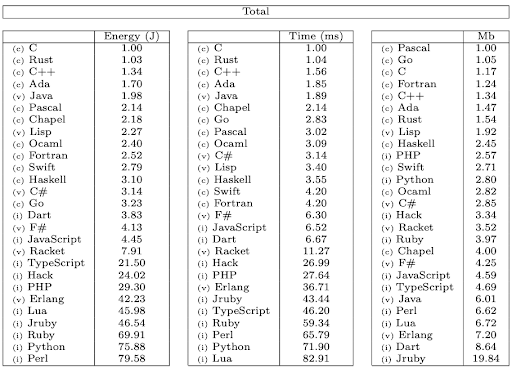
\includegraphics[scale=0.70]{previous-research-languages.png}
	\caption{Normalised global results for Energy, Time, and Memory \cite[p.16]{PEREIRA2021102609}}
	\label{figure:previous-research-languages}
\end{figure}
